\documentclass[twocolumn]{article}
\usepackage{url}
\usepackage{graphicx}

\title{
    Google Analytics Reference Pattern \\
    Investment Products Recommendation Engine \\
    Advanced Analytics White Paper
}
\date{\today}
\author{
    Oleksii Lialka
    \thanks{Staff Data Scientist, SoftServe Inc., olial@softserveinc.com}
}

\begin{document}
\maketitle

\begin{abstract}
    This document provides an overview of the advanced analytics services and solutions of the \emph{Investment Products Recommendation Engine} (IPRE) reference pattern.
    It contains sections dedicated to data pipelines and ETL, advanced analytics and machine learning methodology, principles of the recommendation service.
    The GitHub public repository\footnote{[TBD]: link to GitHub repo} hosts the source code of the IPRE reference pattern.
\end{abstract}

\section{Solution overview}
    The IPRE is a comprehensive investment banking solution, which builds a bridge between retail investors and the complexity of the capital markets.
    The AI/ML products assist clients in optimal portfolio construction, wealth allocation and discovering key performance metrics of the investment.
    An ensemble of ML solutions produces highly personalized recommendations and investment advice based on an individuals' risk preferences and wealth management goals.

    The reference pattern is designed to be highly reproducible, with the minimal manual effort required to set all services up.
    \emph{Terraform} script builds and deploys all components of the IPRE advanced analytics.

\subsection{Project structure}
    The source code of the advanced analytics services is nested under the \verb|advanced-analytics/| directory.
    Scripts content follows a modular structure according to the objectives of ETL, portfolio optimization, investment analytics services.

    Directory \verb|data-pipelines/| contains Cloud Functions scripts for ETL, generating datasets, writing data to Cloud Storage.
    Modules for \emph{capital markets} and \emph{investor risk preferences} datasets have dedicated Cloud Functions for invoking training and inference jobs of BigQuery AutoML and ARIMA models.
    Directory \verb|recommendation-engine/| provides scripts for convex optimization, investment analytics.

\section{Data pipelines}
    The IPRE service relies on multiple data sources, both internal and external.
    The solution implements scalable data pipelines with the Big Data technologies, such as \emph{BigQuery}, \emph{Cloud Storage}, \emph{Dataflow}.
    Data pipelines follow the \emph{schema-on-read} data lake convention.

    All external raw data streams are aggregated in dedicated Cloud Storage buckets.
    The Cloud Functions trigger minor pre-processing scripts.
    Writing an object to the Cloud Storage bucket triggers Dataflow job for adding new data to BigQuery.

    Such architecture makes an ETL pipeline resilient to corrupt data and scalable to multiple data sources.
    The Cloud Functions provide clean, cost-effective solution for migrating massive datasets from data lake to DWH.

\subsection{Capital markets data}
    Historical market data is a crucial element for the recommendation service.
    A dedicated data pipeline job collects quotes of the select securities from \emph{YahooFinance}\footnote{Modular interface of data pipelines permits integration of any other data provider}.
    Securities of interest include the Big Tech stocks, FX, ETF, and others.
    All select assets vary in return and risk.
    It allows IPRE to construct a wide range of portfolios to meet diverse investors' preferences.

    \begin{figure}
        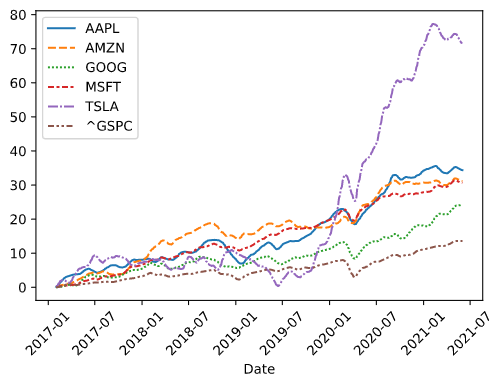
\includegraphics[width=0.49\textwidth]{media/returns-lineplot.png}
        \caption{Cumulative monthly returns of select stocks.}
    \end{figure}

    After minor preprocessing, daily historical quotes ($q$) are turned into periodic \emph{returns}.

    \begin{equation}
        {r_{t, t + dt} = \frac{q_{t + dt} - q_{t}}{q_{t}}}
    \end{equation}

    \emph{Returns} observations with a unique timestamp are written to Cloud Storage.
    It allows to reduce egress and ensures that BigQuery does not receive duplicate data.
    During the first run of the script, all observations starting from 2017 will make it to BigQuery.
    Subsequent runs provide incremental observations of the "unseen" data.

    % Can remove par
    In the final stage of ETL, the processed data is written to BigQuery.
    Aggregating data in BigQuery allows other services to retrieve the data in a cost-effective way.

\subsection{Investors risk preferences}
    The \emph{investor risk preferences} (IRP) is a synthetic dataset containing historical records of 1000 existing retail investors\footnote{The dataset mimics customer data FSI companies typically collect. It can be easily replaced by real clients' data.}.
    This dataset is a crucial component for making personalized recommendations based on an individual's investment preferences.

    \begin{figure}
        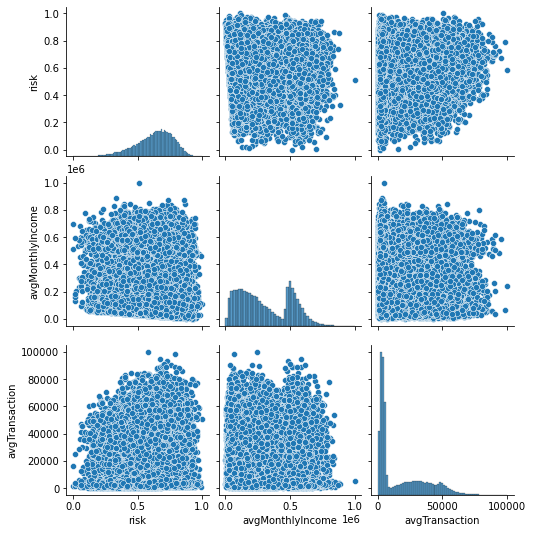
\includegraphics[width=0.49\textwidth]{media/irp-pairplot.png}
        \caption{Pairplot of investor risk preferences select features.}
    \end{figure}

    The \emph{risk aversion} is a target variable of interest.
    \emph{Average monthly income, education, loans, deposits} are among 15 independent variables.
    Investors' attributes are generated using different continuous variable distribution functions: \emph{Gamma, Gumbel, Gaussian, R-distributed and others}.
    A script produces monthly snapshots of investors' attributes, resulting in 48'000 data points.

    The Cloud Function triggers a generation of the dataset upon the first launch of IPRE.
    Dataflow migrates generated dataset from Cloud Storage to BigQuery.

\section{Advanced analytics}
    This section describes the use of BigQuery built-in tools for ML and forecasting.
    The data stored in BigQuery is used for producing factors for the recommendation service.
    BigQuery ML and forecasting tools can also be used for leveraging massive datasets to produce deep customer insights and business analytics.

\subsection{Risk aversion}
    Predicting the risk aversion of prospect investors is a cornerstone IPRE feature.
    The risk aversion factor is a proxy of an investors' risk preference.
    Individuals' risk preference corresponds to the level of risk an investor is comfortable within the long term.
    Modern financial theory and behavioural finance studies advocate that the risk aversion factor shapes the investment decisions of an individual\footnote{Björk, T., Murgoci, A. and Zhou, X.Y. (2014). Mathematical Finance, 24: 1-24.}.

    \begin{figure}
        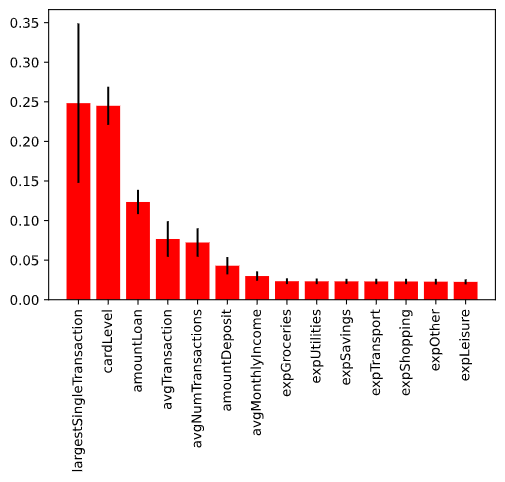
\includegraphics[width=0.49\textwidth]{media/irp-feature-importance.png}
        \caption{Feature importance of the investor risk aversion model.}
    \end{figure}

    Inferring the risk aversion from individuals' attributes is a supervised machine learning problem.
    The Cloud Function invokes script for training BigQuery AutoML model on the IRP data stored in BigQuery.
    BigQuery ML tools handle the entire model training pipeline, from data preparation to hyperparameter tuning.

    \begin{figure}
        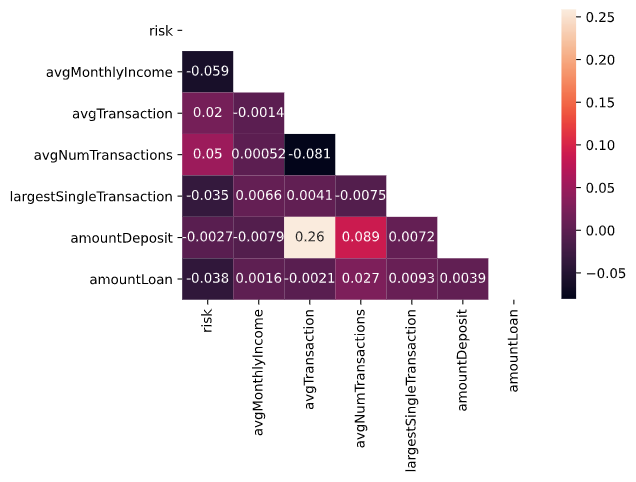
\includegraphics[width=0.49\textwidth]{media/irp-heatmap.png}
        \caption{Correlation map of investor risk preferences select features.}
    \end{figure}

    Once training is complete, an inference script predicts risk aversion for existing clients of the bank, who are not yet active investors.
    The mean objective of the IPRE is to provide non-finance professionals with an insight into individual's risk preferences.

\subsection{Expected returns}
    The IPRE utilizes portfolio optimization technique for producing a recommendation. 
    The expected returns vector ($\mu$) is a predicted return on standalone assets (stocks, indices) in a foreseeable future.
    The precision of the recommendation depends on the accuracy of expected returns.

    Processed historical market quotes turned into periodic returns and stored in BigQuery.
    The Cloud Function triggers the BigQuery forecasting tool to train models for each time series stream.
    Invocation of multi-threaded BigQuery jobs reduces overall training time.
    BigQuery uses an advanced version of \emph{ARIMA} for time series forecasting.
    The BigQuery implementation of \emph{ARIMA} is a good fit for foracasting noisy, non-stationary financial time series data.

    Models make a one-step-ahead prediction of the expected returns and store results in a dedicated Cloud Storage bucket.

\section{Recommendation service}
    The IPRE service takes user ID as an argument, retrieves predicted risk aversion factor, and makes optimal portfolio recommendation.
    The risk aversion factor is inferred from the clients' data using the BigQuery AutoML model.
    The user can select a preferred level of risk with the \emph{UI} to obtain a recommendation, which fits them best.
    The IPRE returns a recommendation on the capital market assets, expected risk, return, portfolio performance metrics.

\subsection{Portfolio optimization}
    The objective of the portfolio optimization is to find a combination of assets, which maximizes the difference between expected return ($\mu$) and a risk ($\Sigma$).
    As far as different investors have different risk preferences, the risk aversion ($\lambda$) introduces a penalty to an objective function.

    \begin{equation}
        \max \: \mu \omega^{T} - \frac{\lambda}{2} \omega^{T} \Sigma \omega \, : \, \forall \: \omega \in \Re
        \label{formula:portfolio}
    \end{equation}

    The higher the risk aversion, the higher the penalty for including risky assets into a portfolio\footnote{MATHEWS, T. (2004). Portfolio Selection with Quadratic Utility Revisited. The Geneva Papers on Risk and Insurance Theory, 29(2), 137-144.}
    Portfolio optimization produces optimal asset weights in the portfolio given risk aversion level.
    User can select a risk aversion factor in the \emph{UI} to obtain a recommendation, which fit them best.

\subsection{Investment analytics}
    The IPRE service computes key performance metrics: expected return, risk and the \emph{Sharpe Ratio}.
    It allows user to make informed decisions on the investments, as well as compare portfolios of different composition.
    As far as high returns are accompanied by high risk, an investor can select a portfolio, which fits their risk appetite.

\section{Implications}
    A risk aversion factor of existing investors can be inferred analytically by solving the first-order condition of the equation (\ref{formula:portfolio}).
    The IPRE can scale to produce recommendations on the OTC assets and structured investment products offered by financial companies to retail investors.
    The BigQuery managed tools for advanced analytics, ML and forecasting allow cost-effectively leverage massive datasets with lower manual effort and maintenance overhead compared to an in-house solution.

    The IPRE unlocks new dimension of \emph{proactive} recommendation engagement.
    Serving professional investment advice via web and mobile interface is a financial services industry differentiator.
    It provides a competitive advantage to a company seeking to increase retail investors' conversion and onboarding rates.
    Providing content-aware, highly personalized recommendations increases the trading activity of existing and prospective retail investors.

\end{document}
